\xchapter{Proposta do trabalho}
{ }%trata-se  da  apresentação  do  estado  em   que  se encontra  o  projeto, dissertando quais são as contribuições esperadas, seguido pelo cronograma de atividades}

% \presetkeys%
%      {todonotes}%
%     {inline,backgroundcolor=yellow}{}

Tendo como estudo de caso o \ac{SAD}, sob a administração do \ac{HHCP} na cidade de Salvador, Bahia, este projeto tem como principal objetivo estudar e analisar a utilização da técnica de Programação por Restrições e propor um modelo para ser aplicada na prática com o intuito de aumentar a quantidade de pacientes atendidos pelo programa e reduzir o tempo gasto pelas equipes de enfermeiras por meio de construção de rotas de visitas mais eficientes. Como contribuições concretas deste trabalho podemos listar:

\begin{enumerate}
\item Elaboração de uma Revisão sistemática de literatura, permitindo uma discussão sobre métodos existentes aplicadas ao \ac{SAD} e auxiliando no processo de obtenção de materiais para pesquisas futuras;
\item Metodologia detalhada, garantindo a reprodutibilidade em trabalhos futuros;
\item Criação de ferramenta prática para o problema do \ac{FESFSUS} que pode ser adaptada para utilização em outros casos de \ac{SAD};
\end{enumerate}

%O \ac{SAD} caracteriza-se como uma modalidade de atenção à saúde composta por um conjunto de ações de prevenção, reabilitação e tratamento de doenças prestadas em domicílio.
%Esse serviço tem se tornado cada vez mais presente como ação de saúde complementar ou substituto à internação hospitalar, pois oferece uma nova modalidade de atendimento às pessoas com quadro clinico estável que necessitam de cuidados.
%Essa modalidade permite maior comodidade aos pacientes, aumentando o conforto e facilitando o apoio familiar, além de auxiliar a reduzir os riscos contaminação hospitalar e reduzir a lotação nos hospitais. 
%A \ac{FESFSUS} é um órgão público, sem fins lucrativos que tem como uma das suas atribuições oferecer serviço de atenção domiciliar a pacientes com médio ou alto grau de complexidade.
%O roteamento e escalonamento da equipe de internação domiciliar ainda é realizado de forma manual no Brasil e em diversos países, por vezes utilizando mais tempo do que o esperado na tarefa de elaborar o escalonamento e o roteamento das equipes e em alguns casos gerando resultados ineficazes.
%Acredita-se que a partir da utilização de heurísticas para a elaboração de escalas de trabalho, e das rotas, serão gerados resultados mais eficientes, e como consequência será possível aumentar a cobertura do programa, assim como sua visibilidade, permitindo a expansão do atendimento a pacientes com baixa complexidade e o aumento o total de pacientes de média ou alta complexidade atendidos.  

%\section{Resultados esperados}

%Como resultados esperados após o fim da pesquisa, temos:

%\begin{itemize}
%\item Revisão sistemática de literatura, permitindo uma discussão sobre heurísticas aplicadas ao \ac{SAD} e auxiliando no processo de obtenção de materiais para pesquisas futuras;
%\item Metodologia detalhada do experimento, garantindo a reprodutibilidade em trabalhos futuros;
%\item Solução heurística para o problema do \ac{FESFSUS} que pode ser adaptada para utilização em outros casos específicos e utilizada em casos gerais;
%\end{itemize}

\section{Metodologia e Métodos}

A metodologia utilizada neste projeto levará em consideração a aplicação da técnica de Programação por Restrições. A Programação por Restrições é uma técnica poderosa para resolver problemas de otimização combinatória que se baseia em uma ampla gama de técnicas de inteligência artificial e pesquisa operacional. A Programação de Restrições é atualmente aplicada com sucesso em vários domínios, como em problemas de escalonamento, planejamento, e roteamento de veículos. A idéia básica na Programação de Restrições é a possibilidade de expressar o problema em forma de restrições lógicas e utilizar um solucionador de restrições de propósito geral para resolvê-las.


A definição clássica de um Problema de Satisfação de Restrição (PSR) pode ser expressado da seguinte forma. Um PSR $\mathcal{P}$ é um tripla $P = (X D, C)$ onde $X $é uma $n$-upla das variáveis $X = (x_1, x_2, ..., x_n)$, $D$ é uma $n$-upla de domínios $D = (D_1, D_2, ..., D_n)$ tal que $x_i \in D_i$, $C$ é uma $t$-upla de restrições $C = (C_1, C_2,. . . , C_t)$. Uma restrição $C_j$ é um par $(R_{S_j}, S_j)$ onde $R_{S_j}$ é um subconjunto do produto cartesiano dos domínios das variáveis em $S_j$. Uma solução para o PSR $\mathcal{P}$ é uma $n$-upla $A = (a_1, a_2, ...,a_n)$ e onde $a_i \in D_i$ e cada Cj são satisfeitos.

% Programação por Restrições consiste em um conjunto finito de restrições contendo conjunções de literais, objetos atômicos comuns sem símbolos de função e restrições sobre um determinado domínio. A Programação por Restrições Lógicas é uma extensão da Programação Lógica, sendo ambas consideradas pertencentes ao paradigma declarativo, dessa forma o programador foca em o que computar ao invés de como computar~\cite{maria:2008}.

%textbf{As restrições lineares} denotam restrições construídas a partir de variáveis
%ujo domínio é dado pelo conjunto dos números reais. Para este tipo de
%estrições têm sido implementados meta-interpretadores de restrições bastante
%ficientes que utilizam o algoritmo Simplex como ponto de partida.

As restrições no conjunto $C$ podem ser classificadas em fortes ou fracas. As restrições fortes são aquelas que devem ser satisfeitas obrigatoriamente; e as restrições fracas formam um conjunto de restrições que devem ser satisfeitas se possível, mas para as quais sabem-se que nem todas poderão ser atendidas.

A partir da análise dos mateiras estudados, foi verificado que o método de Programação por Restrições tem se mostrado eficiente na solução de problemas de escalonamento e de roteamento na áreas da saúde. 

O \ac{SAD} no \ac{FESFSUS} precisa lidar diariamente com as seguintes restrições:

\textbf{Restrições fortes:}
\begin{itemize}
\item Uma enfermeira não pode trabalhar mais de um turno por dia;
\item A demanda de enfermeiras para cada turno deve ser satisfeita durante todo o planejamento;
\item Alguns profissionais de saúde não podem trabalhar simultaneamente.
\end{itemize}
 
\textbf{Restrições flexíveis:}
\begin{itemize}
\item Existe uma limitação para o número de turnos atribuídos as enfermeiras; 
\item Existe uma limitação para a quantidade de dias de folga consecutivos; 
\item Existe um máximo número de dias de trabalho consecutivos;
\item Existe um máximo número de fins-de-semana trabalhados consecutivos;
\item Deve haver um número de dias de folga após uma série de turnos noturnos;
\item Existe um máximo número de fins-de-semana trabalhados em um período de quatro semanas; 
\item Devem ser atribuídos turnos idênticos no fim-de-semana;
\item Uma enfermeira não pode ser atribuída à um turno que demanda mais qualidades do que a mesma possui;
\item Um paciente deve ser atendido sempre pela mesma enfermeira.
\end{itemize}

% A Linguagem de Programação Lógica baseia-se em diversos domínios, destacando-se as restrições booleanas, sobre domínios finitos, sobre intervalos reais e os termos lineares. Outros exemplos incluem listas, conjuntos finitos e árvores.

% \textbf{As restrições booleanas} são tratadas por meta-interpretadores de restrições
% especializados, podendo, no entanto, ser tratadas como um caso particular das
% restrições associadas a domínios finitos para esse problema. Neste último caso
% as variáveis apenas podem tomar dois valores inteiros: 0 (falso) ou 1
% (verdadeiro);

% \textbf{As restrições sobre domínios finitos} são utilizadas em muitas áreas do
% conhecimento. Para satisfação destas restrições usa-se uma combinação de
% técnicas para a preservação de consistência, propagação de valores e pesquisa
% com retrocesso. Cada variável possui associado um conjunto finito de valores
% inteiros, ao qual é dado o nome de domínio da variável. Os valores do domínio
% que levam a inconsistências são removidos do domínio das variáveis durante a
% fase de propagação, enquanto que pela pesquisa se tenta instanciar cada
% variável do problema;

% \textbf{As restrições sobre intervalos reais} são o equivalente das consideradas para os domínios finitos, só que aqui trabalha-se com valores reais em vez de
% valores inteiros. As técnicas de remoção de inconsistências são similares às
% técnicas usadas para os domínios finitos, ou então são baseadas em técnicas
% matemáticas de diferenciação automática ou as séries de Taylor;

% \textbf{As restrições lineares} denotam restrições construídas a partir de variáveis cujo domínio é dado pelo conjunto dos números reais. Para este tipo de
% restrições têm sido implementados meta-interpretadores de restrições bastante
% eficientes que utilizam o algoritmo Simplex como ponto de partida.

\section{Atividades previstas}
%trata-se   da   explicitação   do   modo   como  será desenvolvido o trabalho
Como foi mencionado anteriormente, foi levantada a hipótese de que é possível desenvolver um modelo de programação por restrições para o \ac{SAD} aplicando ao caso específico da equipe de atendimento domiciliar FESFSUS, e assim reduzir o tempo das equipes dentro dos veículos e aumentar a quantidade de atendimentos.

Para validar a nossa hipótese utilizaremos um estudo de caso com o Serviço de Atendimento Domiciliar em Salvador administrado pela \ac{FESFSUS}. Foi realizada uma revisão sistemática de literatura para levantar quais abordagens heurísticas que estão sendo utilizadas atualmente para solucionar o problema de escalonamento e roteamento do \ac{SAD}, e dessa forma, a partir do entendimento de casos já estudados tratar o caso da \ac{FESFSUS} e posteriormente casos mais gerais.

Após o estudo de diversas abordagens levantadas e elaboração da abordagem heurística, serão utilizados dados do próprio projeto estudado e outras bases de dados disponíveis na literatura para fins de comparações experimentais.

\subsection{Cronograma de atividades}

O cronograma seguinte apresenta o desenvolvimento das atividades executadas desde o início da pós-graduação, tendo as atividades representadas a cada mês levado em consideração o período de 24 meses, com início em Novembro de 2016 e final previsto para Outubro de 2018, no qual as disciplinas obrigatórias e optativas, assim como o estágio docente orientado foram realizados no primeiro ano de mestrado, como pode ser visto na Figura \ref{cronograma_atividade}.

%cronograma de atividades
\begin{figure}[H]
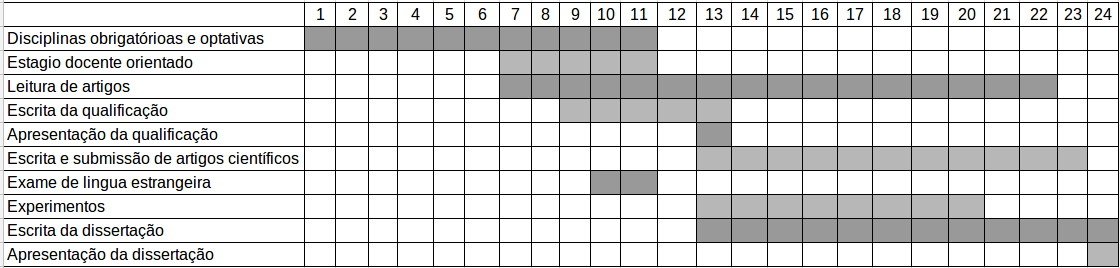
\includegraphics[width=1 \textwidth]{cronograma_atividades.png}
\begin{center}
\caption{Cronograma de atividades previstas. \label{cronograma_atividade}}
%Fonte: Elaborada pelo autor
\end{center}
\end{figure}

